
\chapter{RobotME Framework Design}

We divided the problem into fairly independent goals. The first goal was to design a mechanism
that would allow us to intercept and record the events resulting from user's interaction with the
program (running on an emulator or a real device). This is called the \emph{recording phase}. The 
second goal was to programmatically simulate the previously recorded events (user actions) -- this is
called the \emph{replay phase}. Finally, we compare the initial recording with stimuli 
resulting from the replayed events; certain \emph{assertions} are checked to ensure the program followed
an identical sequence of state transitions (this implies a correct outcome of the entire test). Note
that states can be fairly low-level, such as action selection, but also high-level, perhaps even
explicitly hardcoded in the program under test by the developer. We took extra care to  
facilitate future maintenance of the recorded scripts. Unlike with desktop applications, 
where an event is typically described by a mouse position or some obscure component identifier, 
our events are described with names meaningful to the programmer (an action's label 
for example). Our goal is to make the recorded script comprehensible and comparable to a 
typical (unstructured) use-case scenario used in requirements engineering.


\section{Problems}
% subclassing, finalized classes/ methods, container environment.

The main problem is to capture and generate events of various GUI elements in a consistent, 
reliable manner, regardless of the techniques used by the program developer. We can distinguish
several different scenarios (each explained in detail further on):
\begin{itemize}
    \item \emph{subclassing} used to modify or extend the default behaviour of \texttt{Form}, \texttt{Canvas}, 
    \texttt{MIDlet} and other J2ME elements,
    
    \item \emph{direct use of an object} as in the case of the \texttt{Command} class,
    
    \item \emph{listeners} receiving callback events from \texttt{Form} and other 
    subclasses of \texttt{Displayable}.
\end{itemize}

Additional issues arise from the fact that the above scenarios may appear in different combinations
in the tested program's bytecode -- a bytecode instrumentation solution should detect and properly 
`wrap' such code to capture or generate events.  

Let us provide some more examples of real code and the way it is translated to Java bytecode.

\subsection{A \texttt{Command} object being added to a \texttt{Form}}\label{sect:fiugvuieg}

We must intercept every attempt to add a \texttt{Command} object to an existing screen, namely
the invocation of the \texttt{addCommand} method on \texttt{Displayable}). 
A programmer may add a command in many ways, for example by adding class-level 
static fields:

\begin{javablock}
public class ClassUnderTest {
    private static final Command MY_COMMAND = new Command("Cmd label", Command.OK, 1);

    public ClassUnderTest() {
        Form f = new Form("Title");
        f.addCommand(MY_COMMAND);
    }
}
\end{javablock}

\noindent%
At the bytecode level the above snippet looks as shown below:

\begin{javablock}
ALOAD 1
GETSTATIC ClassUnderTest.MY_COMMAND : Ljavax/microedition/lcdui/Command;
INVOKEVIRTUAL javax/microedition/lcdui/Displayable.addCommand(Ljavax/microedition/lcdui/Command;)V
\end{javablock}

\noindent%
This means: load first local variable onto the stack (\texttt{Form f}), load static class field onto the stack, 
invoke \texttt{addCommand} method of the \texttt{Displayable} instance with the arguments from the stack.
A different attempt to do the same thing is using object-level fields:

\begin{javablock}
public class ClassUnderTest {
    private final Command MY_COMMAND = new Command("Cmd label", Command.OK, 1);

    public ClassUnderTest() {
        Form f = new Form("Title");
        f.addCommand(MY_COMMAND);
    }
}
\end{javablock}

\noindent%
At the bytecode level this translates to:

\begin{javablock}
ALOAD 1
ALOAD 0
GETFIELD ClassUnderTest.MY_COMMAND : Ljavax/microedition/lcdui/Command;
INVOKEVIRTUAL javax/microedition/lcdui/Displayable.addCommand(Ljavax/microedition/lcdui/Command;)V
\end{javablock}

\noindent%
Which means: load first local variable onto the stack (\texttt{Form f}), load `this' variable (self reference) onto the stack,
load object-level field onto the stack (and in the same step remove `this' variable from the stack),
invoke the \texttt{addCommand} method of the \texttt{Displayable} instance with the arguments from the stack.

The second example is only slightly different from the first one. But it is possible to do the same thing in
completely different manner, using factory methods:

\begin{javablock}
public class ClassUnderTest {
    private static final Command getMyCommand() {
        return new Command("Cmd label", Command.OK, 1);
    }

    public ClassUnderTest() {
        Form f = new Form("Title");
        f.addCommand(getMyCommand());
    }
}
\end{javablock}

\noindent%
results in bytecode:

\begin{javablock}
ALOAD 1
INVOKESTATIC ClassUnderTest.getMyCommand()Ljavax/microedition/lcdui/Command;
INVOKEVIRTUAL javax/microedition/lcdui/Displayable.addCommand(Ljavax/microedition/lcdui/Command;)V
\end{javablock}

\noindent%
Yet another alternative is providing \texttt{Command} objects while adding it 
to the \texttt{Form}:

\begin{javablock}
public class ClassUnderTest {
    public ClassUnderTest() {
        Form f = new Form("Title");
        f.addCommand(new Command("Cmd label", Command.OK, 1));
    }
}
\end{javablock}

\noindent%
results in bytecode:

\begin{javablock}
ALOAD 1
NEW javax/microedition/lcdui/Command
DUP
LDC "Cmd label"
ICONST_4
ICONST_1
INVOKESPECIAL javax/microedition/lcdui/Command.<init>(Ljava/lang/String;II)V
INVOKEVIRTUAL javax/microedition/lcdui/Displayable.addCommand(Ljavax/microedition/lcdui/Command;)V
\end{javablock}

A more complex snippet could subclass the \texttt{Command} class (it has no real meaning here, but is
technically correct):

\begin{javablock}
public class ClassUnderTest {
    public ClassUnderTest() {
        Form f = new Form("Title");
        f.addCommand(new Command("Cmd label", Command.OK, 1) {
            public String getLabel() {
                return "Other Cmd label";
            }
        });
    }
}
\end{javablock}

\noindent%
compiles into:

\begin{javablock}
ALOAD 1
NEW ClassUnderTest$1
DUP
ALOAD 0
LDC "Cmd label"
ICONST_4
ICONST_1
INVOKESPECIAL ClassUnderTest$1.<init>(LClassUnderTest;Ljava/lang/String;II)V
INVOKEVIRTUAL javax/microedition/lcdui/Displayable.addCommand(Ljavax/microedition/lcdui/Command;)V
\end{javablock}


\subsection{Subclassing the \texttt{Form} class}

There are also cases that cannot be resolved by simply investigating compiled byte code once because of the complex
interdependencies between the standard API code and code created by the programmer. The only solution then is
having two-phase analysis of the compiled code: the first one creates a map of the interdependencies, and the second
looks for the appropriate injection points. For example, compare creating a \texttt{Form} screen by simply using 
its default constructor:

\begin{javablock}
Form f = new Form("Title");
\end{javablock}

\noindent%
to creating an instance of a derived class: 

\begin{javablock}
public class MyOwnForm extends Form {	
    public MyOwnForm(String s) {
        super(s);
    }
}

MyOwnForm f = new MyOwnForm("Title");
\end{javablock}

\noindent%
Creating the first object at the bytecode level looks like this:

\begin{javablock}
NEW javax/microedition/lcdui/Form
DUP
LDC "Title"
INVOKESPECIAL javax/microedition/lcdui/Form.<init>(Ljava/lang/String;)V
ASTORE 1
\end{javablock}

\noindent%
and creating the second object: 

\begin{javablock}
NEW MyOwnForm
DUP
LDC "Title"
INVOKESPECIAL MyOwnForm.<init>(Ljava/lang/String;)V
ASTORE 1
\end{javablock}

Note the second example has no direct relation with the standard J2ME API, therefore
it is impossible to tell only from this snippet of code what type of object
\texttt{MyOwnForm} really is. In the Java runtime we may use \texttt{instanceof} operation
to verify if \texttt{MyOwnForm} is a subclass of \texttt{Form} but it is impossible to do so while
statically investigating Java bytecode. Hence the need for two passes over bytecode -- one to 
determine inheritance hierarchy, the other for detecting potential event injection points.


\subsection{Injection points related to listeners}

Intercepting the addition and removal of listeners is required because we will need to
forward real GUI events to them after recording and artificially generated 
events at replay. The mechanism of intercepting the calls to \texttt{addCommandListener}
method is very similar to the one described previously in Section~\ref{sect:fiugvuieg},
so we omit its details here. An example of a code fragment adding a `self' object as 
a listener of a \texttt{Form} is given below:

\begin{javablock}
public class MyClass implements CommandListener {
    public MyClass(Form f) {
        f.addCommandListener(this);
    }
...
\end{javablock}


\subsection{Storage for recorded events}

An additional problem to solve in the recording phase was related to storage
of the recorded events. Saving all events directly on the device was inconvenient
because we could collide with the application's data or exceed the device's limited
capacity (memory or persistent storage). Eventually we decided to transmit all
events directly over the wire during the simulation and have an option to save
them locally in case network protocol is unavailable on the device.



\section{High-level Architecture}

When talking about high-level architecture we must distinguish several parts of the framework:

\begin{description}
    \item[Framework core] A group of classes used both during event capturing and
replaying. Contains most of the code that performs event capturing and forwarding 
events to the Log Server module.

    \item[Enhancer] A separate tool that gets as its input Java archive (JAR) file
with the compiled Java mobile applications and returns an `enhanced' version of the bytecode
with injected instructions related to the RobotME Testing Framework. 
It works in two modes: one dedicated to recording/ capturing phase that creates
enhanced JAR with injected code that is able to intercept user events;
second dedicated to replaying phase that creates enhanced JAR with injected code that
is able to simulate previously captured events.

    \item[Log Server] A tool that is deployed on some PC machine and is 
constantly listening for incoming messages from the mobile phone under test. It stores
received messages (events) from the mobile phone in the byte protocol format.

    \item[XML Processor] A tool for decoding the binary protocol
    with stored events and convert it into human-friendly XML form and vice versa.

    \item[Application under test] Not really part of the RobotME Testing Framework but an
    important element of the testing scenario; forms an input to the RobotME Testing Framework.
\end{description}

\begin{figure}[t]%
\begin{center}
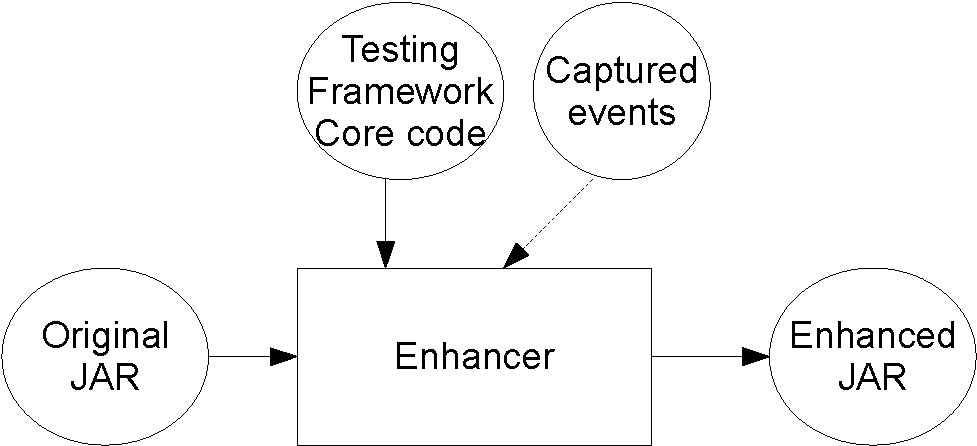
\includegraphics[width=.5\linewidth]{figures/diagram1}
\end{center}
\caption{Enhancement process.}%
\label{fig:diagram1}
\end{figure}

\begin{figure}[t]%
\begin{center}
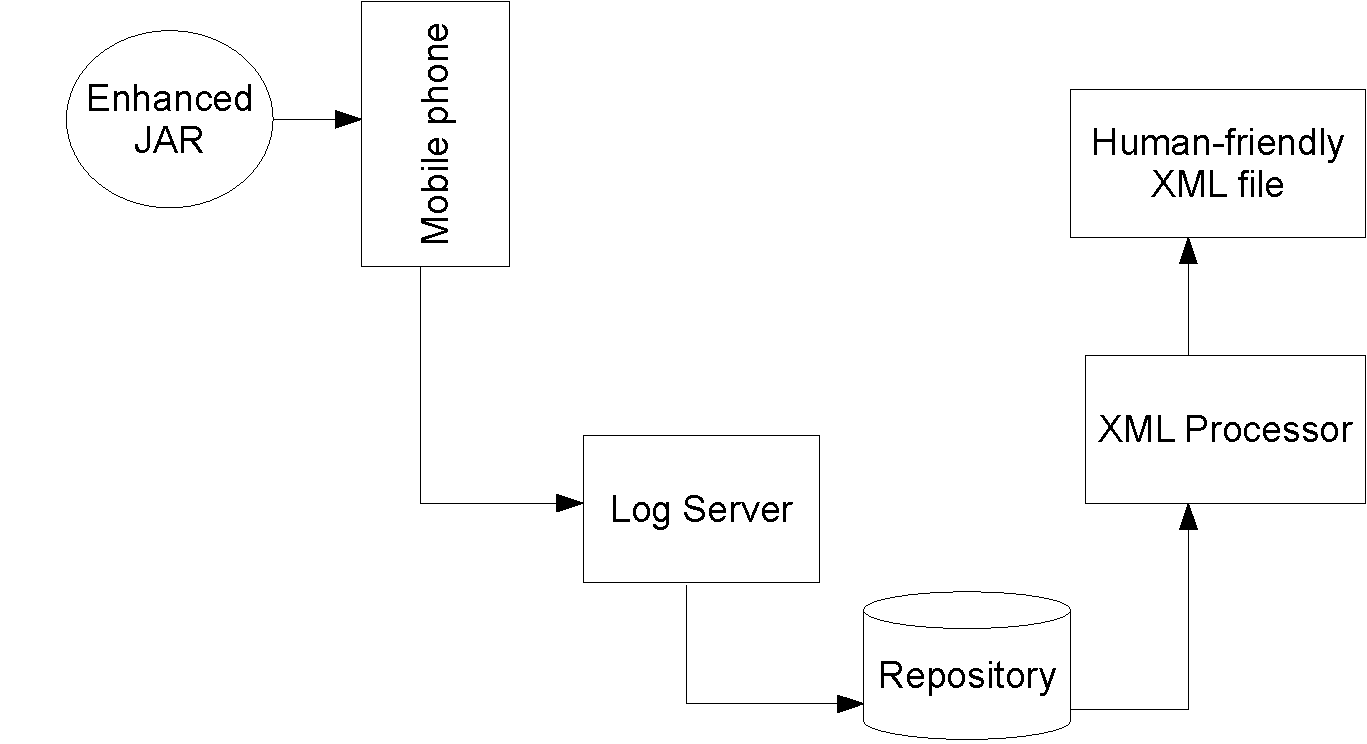
\includegraphics[width=.6\linewidth]{figures/diagram2}
\end{center}
\caption{Typical capturing/ replaying process.}%
\label{fig:diagram2}
\end{figure}

Going into further details of RobotME core architecture  (but still not going into
low-level implementation detail) several most important classes must be described and
interrelations between them. All of the important classes are depicted in 
Figure~\ref{fig:uml-diagram-1}.

\begin{figure}[p]%
\begin{center}
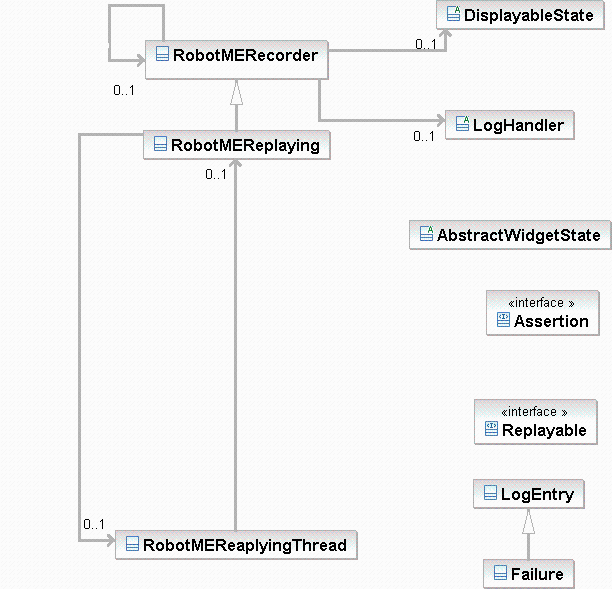
\includegraphics[width=\linewidth]{figures/uml-diagram-1}
\end{center}
\caption{Most important classes from RobotME core.}%
\label{fig:uml-diagram-1}
\end{figure}

\begin{description}
\item[RobotMERecorder] It is the central point of all of the framework activities and the only class
that is directly invoked from the injected code. It preserves all important information
about  the running Midlet like: connections between displaying screens and commands on them
and what screen is currently displayed.

\item[RobotMEReplaying] This class derives from the \texttt{RobotMERecorder} class because from the
capture-replay framework point of view replaying process is an extended version of recording process.
It is because during replaying process to be able to watch what is going on in the application
we must observe the application, therefor record each occurred events. Note that \texttt{RobotMEReplaying}
is used only during replaying process, but \texttt{RobotMERecorder} is used both during capturing
and replaying process. The important parts in which this class extend \texttt{RobotMERecorder} class
is mostly by adding ability of starting and stopping replaying process.

\item[RobotMEReaplyingThread] it is usual Java thread (derives from standard \texttt{Thread} class).
The responsibility of this class is to constantly read remaining events from the repository
(usually repository is plain file located in the same JAR as Midlet application) and simulate read events in
appropriate time intervals.

\item[DisplayableState] it is common knowledge that all action usually has some reaction (visible or not).
The same is with mobile application: all user or system-level actions (events) usually leads to some
reaction (both visible on the screen but not always). \texttt{DisplayableState} abstract class is the
way of storing all those reactions that are visible on the screen. There are many implementations
of this class: \texttt{AlertState}, \texttt{CanvasState}, \texttt{FormState}, 
\texttt{ListState} and \texttt{TextBoxState}. All screen
types existing in J2ME specification has its own \texttt{DisplayableState} implementation that
knows how to obtain and preserve state of such a screen.

\item[AbstractWidgetState] one of the screen types could have very complex internal state -- it is the
\texttt{Form} screen.
This kind of screen has its own implementation of \texttt{DisplayableState} -- a \texttt{FormState} class.
\texttt{FormState} implementation preserves only general information about \texttt{Form},
like its title and ticker text
(ticker is kind of scroll bar that is constantly scrolling some text on top or on the 
bottom of mobile phone screen). Forms as defined in the J2ME specification could have
so-called \texttt{Items} in it. The examples of predefined items are: simple labels, text fields, data fields,
choice groups (radio buttons or check-boxes), gauges, images and more, even custom items
(prepared entirely by the programmer, in current prototype implementation our testing
framework does not support this kind custom of Items). Each of this items has its own internal state, and
taken together form state of their parent Form. AbstractWidgetState abstract class
is the parent class for all of the implementations that store information
about internal states of the items. Some of the implementations are:
\texttt{ChoiceGroupWidgetState}, \texttt{DateFieldWidgetState}, \texttt{ImageItemWidgetState},
\texttt{TextFieldWidgetState} and
others. Each of implementation of \texttt{AbstractWidgetState} knows how to retrieve state
of its Item and how to preserve it (serialize to the event code).

\item[LogHandler] is the handler responsible for logs, for forwarding serialized events to appropriate
receiver. Examples of such receivers could be: remote PC with socket, bluetooth, infra-red
or serial connection, or even local (on the phone) receiver that stores events in the local
store (so called Record Store).

\item[LogEvent] is the base class for all kind of events possible to intercept during
program execution. Detailed list of every event types is presented in the next section.

\item[Replayable] is a base interface for implementation of class that are able to
simulate (replay) previously recorded events.

\item[Assertion] after each of simulated action state of the whole application is verified
(display screen, internal memory etc). This kind of verification is called assertion,
and if the verification process does not succeed Failure event is stored as the 
occurred event (it is kind of internal special purposes event).

\end{description}


\section{Recorded Event Types}

RobotME Testing Framework was created with the possibility of easily extending events set in mind.
In the current prototype implementation we were concentrated on implementing interception of most
occurred events, which are:
\begin{itemize}
\item  intercepting of modification of every kind of screens, also with complex 
\texttt{Canvas} and \texttt{Forms} (excluding custom items inside forms,
 it is possible to support such kind of items, but needs to introduce direct dependency between
 application under test and RobotME Testing Framework,
 it is subject to future extends),
\item  intercepting invocation of Commands actions,
\item  intercepting of low-level key events,
\item  intercepting of low-level pointer events.
\end{itemize}

This set of interceptors allows to test most of the currently existing mobile applications.

The other kind of interceptors that are planned to implement in the future:
\begin{itemize}
\item  intercepting modifications of the local record store,
\item  intercepting invocations of all phone calls,
\item  intercepting incoming and outgoing SMS, MMS i CBS messages,
\item  intercepting incoming and outgoing HTTP, socket, bluetooth and other kind of connections,
\item  intercepting sound events,
\item  intercepting every access to \texttt{System.out} and \texttt{System.err} streams.
\end{itemize}

Most of mobile phone hardware vendors have their own API to fulfill special needs like: LED lighting,
access to vibra or mobile phone contact book. We are not considering implementation of such
proprietary events, but left our RobotME Testing Framework open and it will be possible to
implement such events by the interested in them parties as a future extends.
